\documentclass{article}
\usepackage{pgfplots}
\pgfplotsset{compat=1.17}

\begin{document}

\begin{figure}[h]
    \centering
    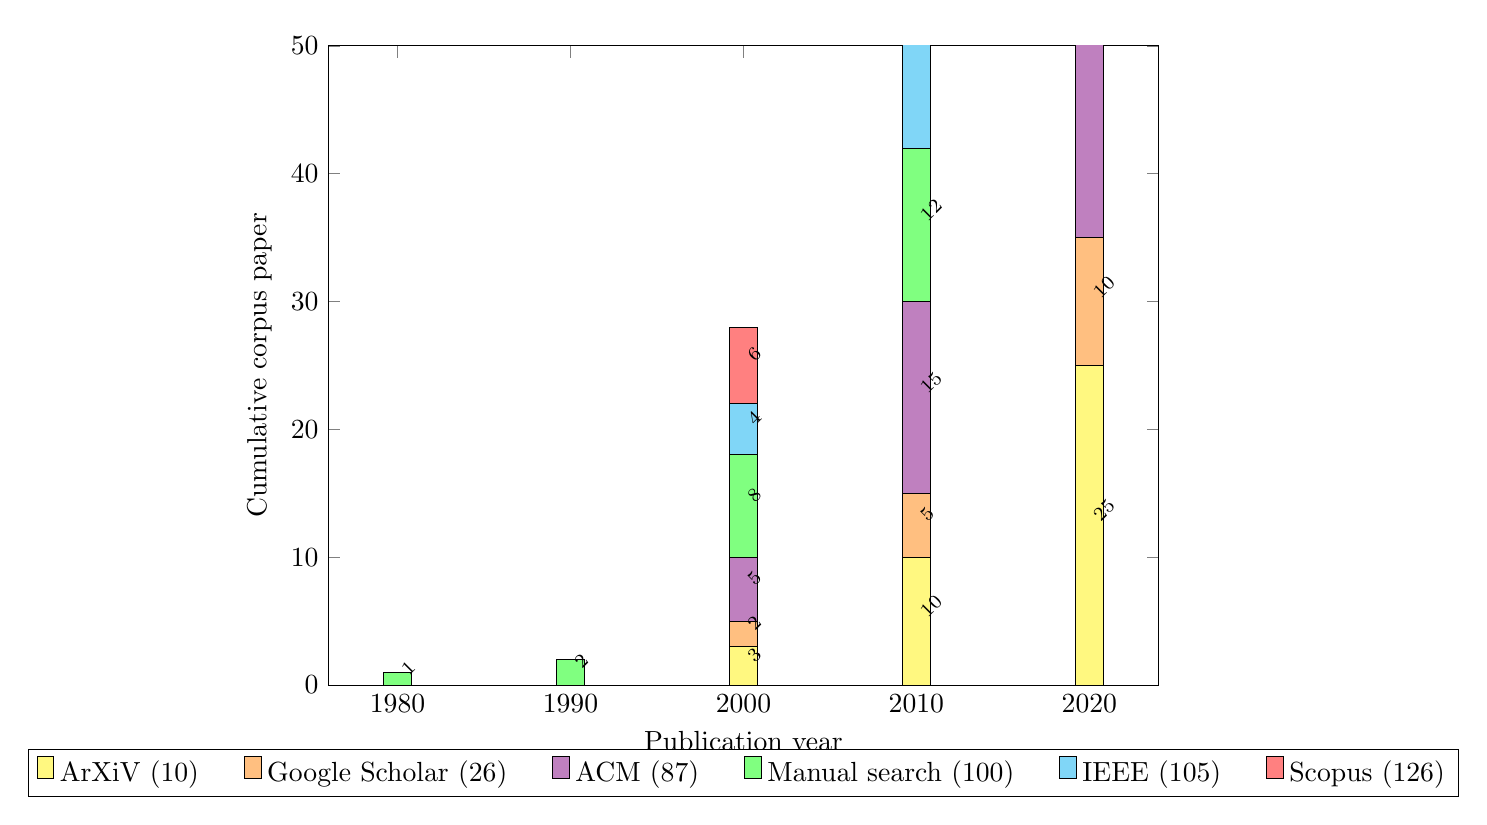
\begin{tikzpicture}
        \begin{axis}[
            width=\textwidth,
            height=0.8*\textwidth,
            xlabel={Publication year},
            ylabel={Cumulative corpus paper},
            ybar stacked,
            ymin=0,
            ymax=50,
            xtick=data,
            xticklabels={1980, 1990, 2000, 2010, 2020},
            legend style={
                at={(0.5,-0.1)},
                anchor=north,
                legend columns=-1,
                /tikz/every even column/.append style={column sep=0.5cm}
            },
            nodes near coords,
            every node near coord/.append style={
                anchor=west,
                rotate=45,
                /pgf/number format/1000 sep=,
                font=\scriptsize
            }
        ]
            \addplot[fill=yellow!50] coordinates {
                (1980,0) (1990,0) (2000,3) (2010,10) (2020,25)
            };
            \addplot[fill=orange!50] coordinates {
                (1980,0) (1990,0) (2000,2) (2010,5) (2020,10)
            };
            \addplot[fill=violet!50] coordinates {
                (1980,0) (1990,0) (2000,5) (2010,15) (2020,30)
            };
            \addplot[fill=green!50] coordinates {
                (1980,1) (1990,2) (2000,8) (2010,12) (2020,20)
            };
            \addplot[fill=cyan!50] coordinates {
                (1980,0) (1990,0) (2000,4) (2010,10) (2020,15)
            };
            \addplot[fill=red!50] coordinates {
                (1980,0) (1990,0) (2000,6) (2010,10) (2020,15)
            };

            \legend{ArXiV (10), Google Scholar (26), ACM (87), Manual search (100), IEEE (105), Scopus (126)}
        \end{axis}
    \end{tikzpicture}
    \caption{Cumulative corpus papers by publication year.}
    \label{fig:sample_69}
\end{figure}

\end{document}